% Reviewed translation: PDF pages 194--200 / printed pages 180--186.
% Continues the proof of Theorem 4.2 from the preceding file.
\MathBookSourcePage{194}
$q\in H^1(\Omega_r)\cap L_0^2(\Omega_r)$ 替换为 $\bar q$ 来处理, 其中
\[
\widehat{\bar q}=\widehat q-\frac1{\operatorname{meas}(\widehat\Omega)}
\int_{\widehat\Omega}\widehat q\,d\widehat x.
\]
于是 $q$ 与 $\bar q$ 相差一个常数, 且
\[
\|q\|_{0,\Omega_r}
=\inf_{c\in\mathbb R}\|q+c\|_{0,\Omega_r}
\leq\|\bar q\|_{0,\Omega_r}.
\]
但
\[
\begin{aligned}
\|\bar q\|_{0,\Omega_r}^2
&=\sum_{i=1}^J\operatorname{meas}(\kappa_i)
\|\widehat{\bar q}\|_{0,\widehat\kappa_i}^2\\
&\leq\widehat C_7\sup_{1\leq i\leq J}(h_{\kappa_i}^2)
|\widehat q|_{1,\widehat\Omega}^2,
\qquad
\widehat q\in H^1(\widehat\Omega)\cap L_0^2(\widehat\Omega),\\
&\leq\widehat C_8
\left\{\frac{\sup_{1\leq i\leq J}(h_{\kappa_i}^2)}
{\inf_{1\leq i\leq J}(\rho_{\kappa_i}^2)}\right\}
\sum_{i=1}^J\operatorname{meas}(\kappa_i)
|\widehat q|_{1,\widehat\kappa_i}^2.
\end{aligned}
\]
因此
\begin{equation}\label{eq:primitive-hood-taylor-reference-poincare}
\left\{\sum_{i=1}^J\operatorname{meas}(\kappa_i)
|\widehat q|_{1,\widehat\kappa_i}^2\right\}^{1/2}
\geq(\widehat C_9/\sigma_r)\|q\|_{0,\Omega_r},
\end{equation}
其中
\[
\sigma_r=\frac{\sup_{1\leq i\leq J}h_{\kappa_i}}
{\inf_{1\leq i\leq J}\rho_{\kappa_i}}.
\]
这就完成了证明, 因为 $\mathcal T_h$ 的正则性蕴含(参见 Bernardi)
\begin{equation}\label{eq:primitive-hood-taylor-macroelement-shape-bound}
\sigma_r\leq\widehat C\sigma.
\end{equation}
\end{Proof}

由 Theorem~\ref{thm:primitive-local-to-global-inf-sup}, 局部 inf-sup 条件
\eqref{eq:primitive-hood-taylor-local-inf-sup} 立即给出所需的整体条件.

\setcounter{statement}{0}
\renewcommand{\theHstatement}{corollary.\thesection.\arabic{statement}}
\begin{Corollary}\label{cor:primitive-hood-taylor-global-inf-sup}
在 Theorem~\ref{thm:primitive-hood-taylor-local-inf-sup} 的假设下,
由 \eqref{eq:primitive-hood-taylor-velocity-space} 和
\eqref{eq:primitive-continuous-linear-pressure-spaces} 定义的空间对
$(X_h,M_h)$ 满足 inf-sup 条件
\eqref{eq:primitive-continuous-pressure-inf-sup}, 其中常数 $\beta^*>0$
与 $h$ 无关.
\end{Corollary}

\begin{Proof}
令 $\overline X_h$ 为 \eqref{eq:primitive-bernardi-raugel-velocity-spaces}
定义的有限元空间, 并令
\[
\overline M_h=\{q\in L_0^2(\Omega);
\ q|_{\Omega_r}\text{ 为常数 }\forall r\}.
\]
一方面, $\overline X_h\subset X_h$, 因为 $\overline X_h$ 中的函数是分片
不完全 $P_2^2$ 多项式. 另一方面, Lemma
\ref{lem:primitive-bernardi-raugel-fortin-estimates} 表明空间对
$(\overline X_h,\overline M_h)$ 满足一致 inf-sup 条件, 因为
$\overline M_h$ 中的函数是分片常数的一种特殊情形. 因而结论由
Theorems~\ref{thm:primitive-local-to-global-inf-sup} 和
\ref{thm:primitive-hood-taylor-local-inf-sup} 得到.
\end{Proof}

\MathBookSourcePage{195}
\setcounter{statement}{0}
\renewcommand{\theHstatement}{remark.\thesection.\arabic{statement}}
\begin{Remark}\label{rem:primitive-hood-taylor-proof-comparison}
Theorem~\ref{thm:primitive-hood-taylor-local-inf-sup} 证明中的大部分技术细节,
Bercovier \& Pironneau 在建立 inf-sup 条件
\eqref{eq:primitive-continuous-pressure-inf-sup} 的一个弱形式时已经使用过.
上述证明虽简单却很长, 因为它处理的参考区域由多个参考三角形组成, 而不是
单个参考三角形. 证明的关键点是在内部线段中点处对 $\mathbf v$ 的特殊选择.
除此以外, 主要步骤与证明 Theorem~\ref{thm:primitive-triangle-local-inf-sup}
时所用步骤基本相同.
\end{Remark}

由 Theorem~\ref{thm:primitive-hood-taylor-local-inf-sup} 及其 Corollary,
立即得到本小节的主要结果.

\setcounter{statement}{2}
\renewcommand{\theHstatement}{theorem.\thesection.\arabic{statement}}
\begin{Theorem}\label{thm:primitive-hood-taylor-error}
设 $\Omega$ 是有界平面多边形, 且 Stokes 系统
\eqref{eq:primitive-continuous-pressure-stokes-system} 的解 $(\mathbf u,p)$ 满足
\[
\mathbf u\in[H^{k+1}(\Omega)\cap H_0^1(\Omega)]^2,
\qquad p\in H^k(\Omega)\cap L_0^2(\Omega),
\qquad k=1\text{ 或 }2.
\]
若三角剖分 $\mathcal T_h$ 正则并满足
\eqref{eq:primitive-hood-taylor-macroelement-partition}, 则使用分别由
\eqref{eq:primitive-hood-taylor-velocity-space} 和
\eqref{eq:primitive-continuous-linear-pressure-spaces} 定义的空间 $X_h,M_h$ 时,
问题 \eqref{eq:primitive-continuous-pressure-discrete-problem} 的解
$(\mathbf u_h,p_h)$ 满足
\begin{equation}\label{eq:primitive-hood-taylor-h1-pressure-error}
|\mathbf u-\mathbf u_h|_{1,\Omega}+\|p-p_h\|_{0,\Omega}
\leq C_1h^k\{\|\mathbf u\|_{k+1,\Omega}+|p|_{k,\Omega}\},
\qquad k=1\text{ 或 }2.
\end{equation}
当 $\Omega$ 为凸集时, 该结果可改进为
\begin{equation}\label{eq:primitive-hood-taylor-l2-error}
\|\mathbf u-\mathbf u_h\|_{0,\Omega}
\leq C_2h^{k+1}\{\|\mathbf u\|_{k+1,\Omega}+|p|_{k,\Omega}\}.
\end{equation}
此外, 若 $\mathcal T_h$ 一致正则(但 $\Omega$ 不必为凸集), 还有
\begin{equation}\label{eq:primitive-hood-taylor-pressure-h1-error}
|p-p_h|_{1,\Omega}
\leq C_3h^{k-1}\{\|\mathbf u\|_{k+1,\Omega}+|p|_{k,\Omega}\}.
\end{equation}
\end{Theorem}

\setcounter{statement}{1}
\renewcommand{\theHstatement}{remark.\thesection.\arabic{statement}}
\begin{Remark}\label{rem:primitive-hood-taylor-pressure-h1-proof}
为建立 \eqref{eq:primitive-hood-taylor-pressure-h1-error}, 可应用
Corollary~\ref{cor:primitive-hood-taylor-global-inf-sup}, 再由
Corollary~\ref{cor:appendix-global-inverse-gradient} 把
$\|p_h-q_h\|_{0,\Omega}$ 换成 $|p_h-q_h|_{1,\Omega}$
(这正是需要 $\mathcal T_h$ 一致正则之处).
\end{Remark}

\setcounter{statement}{2}
\renewcommand{\theHstatement}{remark.\thesection.\arabic{statement}}
\begin{Remark}\label{rem:primitive-hood-taylor-rough-regularity}
显然, Remark~\ref{rem:primitive-triangle-higher-rough-convergence} 在这里也成立.
\end{Remark}

最后快速考察 Hood--Taylor 方法的一个常用变体. 仍设 $\mathcal T_h$ 是满足
\eqref{eq:primitive-hood-taylor-macroelement-partition} 的 $\Omega$ 的正则三角剖分,
并连接每个三角形 $\kappa$ 的边中点, 将其分为四个相等的子三角形
$\widetilde\kappa$(参见 Figure~\ref{fig:primitive-hood-taylor-refined-triangle}).
压力仍采用 \eqref{eq:primitive-continuous-linear-pressure-spaces} 定义的
空间 $Q_h,M_h$, 而把速度空间 $X_h$ 替换为
\begin{equation}\label{eq:primitive-hood-taylor-refined-velocity-space}
X_h=\{\mathbf v\in C^0(\overline\Omega)^2;
\ \mathbf v|_{\widetilde\kappa}\in P_1^2
\text{ 对每个 }\kappa\in\mathcal T_h\text{ 的每个子三角形 }
\widetilde\kappa,\ \mathbf v|_\Gamma=\mathbf0\}.
\end{equation}
$Q_h,M_h$ 的逼近性质不变, 而 $X_h$ 的逼近性质对应于 $P_1$ 多项式, 即
\begin{equation}\label{eq:primitive-hood-taylor-refined-interpolation-error}
\|\mathbf v-I_h\mathbf v\|_{m,\Omega}
\leq Ch^{2-m}|\mathbf v|_{2,\Omega}
\qquad\forall\mathbf v\in H^2(\Omega)^2,
\quad m=0\text{ 或 }1,
\end{equation}

\MathBookSourcePage{196}
其中
$I_h\in\mathcal L([H^2(\Omega)\cap H_0^1(\Omega)]^2;X_h)$
是在 $\mathcal T_h$ 每个子三角形 $\widetilde\kappa$ 的顶点处定义的标准插值算子.

\begin{figure}[htbp]
\centering
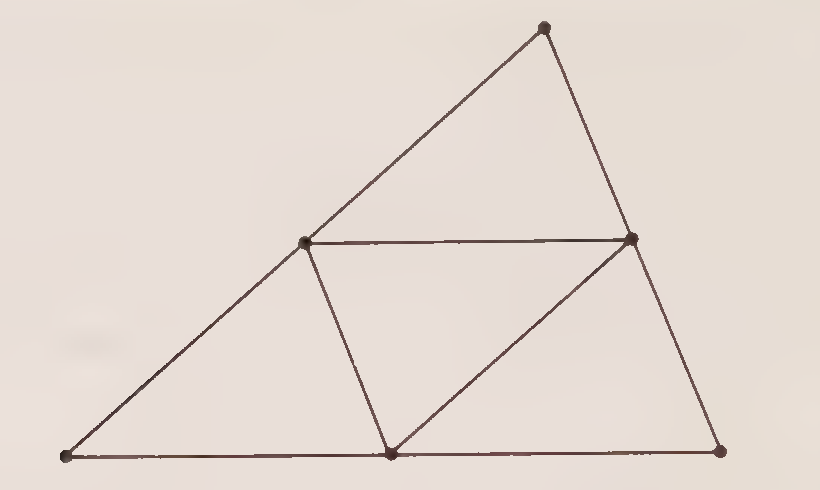
\includegraphics[width=.52\linewidth]{figures/chapter-02-figure-19.png}
\caption{三角形 $\kappa$ 分成四个子三角形.}
\label{fig:primitive-hood-taylor-refined-triangle}
\end{figure}

inf-sup 条件的证明与上面几乎完全相同. 取同一分割
\eqref{eq:primitive-hood-taylor-macroelement-partition}, 并注意, 当 $X_h$
由 \eqref{eq:primitive-hood-taylor-refined-velocity-space} 定义时,
$X_h(\Omega_r)$ 中所涉及的自由度与 $X_h$ 由
\eqref{eq:primitive-hood-taylor-velocity-space} 定义时完全相同. 只有多项式次数
发生变化, 而这仅影响求积公式
\eqref{eq:primitive-hood-taylor-local-quadrature} 中的因子 $1/3$, 以及后续公式中的
参考常数 $\widehat C$. 因而 Theorem
\ref{thm:primitive-hood-taylor-local-inf-sup} 的陈述在此不作修改仍然成立.

为了从局部 inf-sup 条件转到整体 inf-sup 条件, 取同一空间 $\overline M_h$,
但令 $\overline X_h=X_h$. 容易证明空间对
$(\overline X_h,\overline M_h)$ 满足一致 inf-sup 条件. 事实上, 这是下列更一般
结果的一部分.

\setcounter{statement}{1}
\renewcommand{\theHstatement}{lemma.\thesection.\arabic{statement}}
\begin{Lemma}\label{lem:primitive-refined-p1-p0-inf-sup}
若三角剖分 $\mathcal T_h$ 正则, 则空间 $X_h$ 与
\[
\{q\in L_0^2(\Omega);\ q|_\kappa\text{ 为常数 }
\ \forall\kappa\in\mathcal T_h\}
\]
满足一致 inf-sup 条件.
\end{Lemma}

证明略去, 因为它已经包含在 Lemma
\ref{lem:primitive-q1-p0-supermacro-global-inf-sup} 的论证中: 只需把限制算子
$\pi$ 的定义改写为当前情形.

概括上述结果, 得到 Theorem~\ref{thm:primitive-hood-taylor-error} 的对应形式.

\setcounter{statement}{3}
\renewcommand{\theHstatement}{theorem.\thesection.\arabic{statement}}
\begin{Theorem}\label{thm:primitive-refined-p1-p1-error}
设 $\Omega$ 和 $\mathcal T_h$ 满足 Theorem
\ref{thm:primitive-hood-taylor-error} 的假设, 并设
\eqref{eq:primitive-continuous-pressure-stokes-system} 的解 $(\mathbf u,p)$ 属于
$H^2(\Omega)^2\times[H^1(\Omega)\cap L_0^2(\Omega)]$.
则使用分别由 \eqref{eq:primitive-hood-taylor-refined-velocity-space} 和
\eqref{eq:primitive-continuous-linear-pressure-spaces} 定义的 $X_h,M_h$ 时,
问题 \eqref{eq:primitive-continuous-pressure-discrete-problem} 的解
$(\mathbf u_h,p_h)$ 满足
\begin{equation}\label{eq:primitive-refined-p1-p1-h1-error}
|\mathbf u-\mathbf u_h|_{1,\Omega}+\|p-p_h\|_{0,\Omega}
\leq C_1h\{\|\mathbf u\|_{2,\Omega}+|p|_{1,\Omega}\}.
\end{equation}
此外, 当 $\Omega$ 为凸集时, 有 $L^2$ 估计
\begin{equation}\label{eq:primitive-refined-p1-p1-l2-error}
\|\mathbf u-\mathbf u_h\|_{0,\Omega}
\leq C_2h^2\{\|\mathbf u\|_{2,\Omega}+|p|_{1,\Omega}\}.
\end{equation}
\end{Theorem}

\MathBookSourcePage{197}
\setcounter{statement}{3}
\renewcommand{\theHstatement}{remark.\thesection.\arabic{statement}}
\begin{Remark}\label{rem:primitive-refined-p1-p1-conditioning}
尽管最后这个方法包含相同数量的未知量, 精度却低于前一个格式, 但它通常更受
青睐, 因为它得到的线性方程组条件更好.
\end{Remark}

\subsection{``Glowinski--Pironneau'' 有限元方法}
\label{subsec:primitive-glowinski-pironneau}

先设维数 $N$ 为 $2$ 或 $3$. 本小节讨论的数值格式由
Glowinski \& Pironneau 引入, 它以压力的 Poisson 方程为基础. 对方程
\[
-\nu\Delta\mathbf u+\operatorname{grad}p=\mathbf f
\]
两边取散度, 并利用条件 $\operatorname{div}\mathbf u=0$, 得
\[
\Delta p=\operatorname{div}\mathbf f\quad\text{in }\Omega.
\]
因而, 若已知 $p$ 在 $\Gamma$ 上的迹 $\rho=p|_\Gamma$, 则 Stokes 方程组
化为 Laplace 算子的 $N+1$ 个 Dirichlet 问题:
\begin{equation}\label{eq:primitive-gp-pressure-dirichlet}
\Delta p=\operatorname{div}\mathbf f\quad\text{in }\Omega,
\qquad p=\rho\quad\text{on }\Gamma,
\end{equation}
\begin{equation}\label{eq:primitive-gp-velocity-dirichlet}
\nu\Delta\mathbf u=\operatorname{grad}p-\mathbf f\quad\text{in }\Omega,
\qquad\mathbf u=\mathbf0\quad\text{on }\Gamma.
\end{equation}
事实上, $\rho$ 是问题的主要未知量. 我们将说明, $\rho$ 又可由约束
$\operatorname{div}\mathbf u=0$ 确定.

更精确地, 注意 $\mathbf u,p$ 可分解成两个分量:
\begin{equation}\label{eq:primitive-gp-splitting}
\mathbf u=\mathbf u^0+\mathbf u(\rho),
\qquad p=p^0+p(\rho),
\end{equation}
其中 $p^0,\mathbf u^0$ 是 Dirichlet 问题
\begin{subequations}\label{eq:primitive-gp-zero-boundary-problems}
\begin{align}
\Delta p^0&=\operatorname{div}\mathbf f\quad\text{in }\Omega,
&p^0&=0\quad\text{on }\Gamma,\label{eq:primitive-gp-zero-pressure}\\
\nu\Delta\mathbf u^0&=\operatorname{grad}p^0-\mathbf f\quad\text{in }\Omega,
&\mathbf u^0&=\mathbf0\quad\text{on }\Gamma,
\label{eq:primitive-gp-zero-velocity}
\end{align}
\end{subequations}
的解; 对每个边界值 $g$, $p(g),\mathbf u(g)$ 是
\begin{subequations}\label{eq:primitive-gp-harmonic-lifting-problems}
\begin{align}
\Delta p(g)&=0\quad\text{in }\Omega,
&p(g)&=g\quad\text{on }\Gamma,
\label{eq:primitive-gp-harmonic-pressure}\\
\nu\Delta\mathbf u(g)&=\operatorname{grad}p(g)\quad\text{in }\Omega,
&\mathbf u(g)&=\mathbf0\quad\text{on }\Gamma
\label{eq:primitive-gp-harmonic-velocity}
\end{align}
\end{subequations}
的解. 选取边界函数 $g$ 的空间 $G$, 使由
\eqref{eq:primitive-gp-harmonic-pressure} 定义的映射
$g\mapsto p(g)$ 是 $G$ 到空间
\[
\{q\in L^2(\Omega);\ \Delta q=0\}
\]
上的同构.

由于 \eqref{eq:primitive-gp-pressure-dirichlet}--
\eqref{eq:primitive-gp-velocity-dirichlet} 的解 $\mathbf u$ 必须满足
\[
\Delta(\operatorname{div}\mathbf u)=0\quad\text{in }\Omega,
\]
约束 $\operatorname{div}\mathbf u=0$ 可表示为
\MathBookSourcePage{198}
\[
(\operatorname{div}\mathbf u,p(g))=0\qquad\forall g\in G,
\]
或等价地表示为
\begin{equation}\label{eq:primitive-gp-boundary-equation}
(\operatorname{div}\mathbf u(\rho),p(g))
=-(\operatorname{div}\mathbf u^0,p(g))
\qquad\forall g\in G.
\end{equation}
下面将看到, 适当选择空间 $G$ 后, 方程
\eqref{eq:primitive-gp-boundary-equation} 确定唯一的边界函数 $\rho$.

为选择 $G$, 将问题 \eqref{eq:primitive-gp-harmonic-pressure} 写成变分形式.
暂时假定函数 $p(g)$ 足够光滑, Green 公式给出
\begin{equation}\label{eq:primitive-gp-harmonic-variational}
\int_\Omega p(g)\Delta\mu\,dx
=\int_\Gamma g\frac{\partial\mu}{\partial n}\,ds
\qquad\forall\mu\in H^2(\Omega)\cap H_0^1(\Omega).
\end{equation}
当边界 $\Gamma$ 是 $C^{1,1}$ 时, Theorem
\ref{thm:normal-derivative-trace} 表明映射
$\mu\mapsto\partial\mu/\partial n$ 从
$H^2(\Omega)\cap H_0^1(\Omega)$ 连续映上 $H^{1/2}(\Gamma)$.
当 $\Gamma$ 是由线段 $\Gamma_j$, $1\leq j\leq J$, 构成的平面多边形时,
Remark~\ref{rem:polygon-boundary-traces} 表明映射
$\mu\mapsto(\partial\mu/\partial n_j;1\leq j\leq J)$ 从
$H^2(\Omega)\cap H_0^1(\Omega)$ 连续映上
$\prod_{1\leq j\leq J}H^{1/2}(\Gamma_j)$. 这些考虑提示选取
\begin{equation}\label{eq:primitive-gp-boundary-space}
G=\left\{
\begin{aligned}
[H^{1/2}(\Gamma)]'&=H^{-1/2}(\Gamma),
&&\Gamma\text{ 为 }C^{1,1},\\
\left[\prod_{1\leq j\leq J}H^{1/2}(\Gamma_j)\right]',
&&&\Gamma\text{ 为二维多边形},
\end{aligned}
\right.
\end{equation}
并赋予它通常的对偶范数; 为简便起见, 两种情形均记为
$\|\cdot\|_{-1/2,\Gamma}$. 当 $g,p(g)$ 由
\eqref{eq:primitive-gp-harmonic-variational} 联系时, 两种情形下都有
\[
\begin{aligned}
\|g\|_{-1/2,\Gamma}
&\leq C_1\sup_{\mu\in H^2(\Omega)\cap H_0^1(\Omega)}
\frac{\int_\Gamma g\,\partial\mu/\partial n\,ds}{\|\mu\|_{2,\Omega}}\\
&\leq\sqrt N C_1\|p(g)\|_{0,\Omega}.
\end{aligned}
\]
反过来, 若 $\Gamma$ 为 $C^{1,1}$, 或 $\Omega$ 是凸多边形, 则由
Remark~\ref{rem:laplace-isomorphism-convex-domain}, 对每个 $q\in L^2(\Omega)$,
问题
\[
\Delta\mu=q\quad\text{in }\Omega,
\qquad\mu=0\quad\text{on }\Gamma
\]
在 $H^2(\Omega)\cap H_0^1(\Omega)$ 中有唯一解, 且
$\|\mu\|_{2,\Omega}\leq C_2\|q\|_{0,\Omega}$. 因此问题
\eqref{eq:primitive-gp-harmonic-variational} 有唯一解 $p(g)$, 并且
\[
\begin{aligned}
\|p(g)\|_{0,\Omega}
&\leq C_2\sup_{\mu\in H^2(\Omega)\cap H_0^1(\Omega)}
\frac{\int_\Omega p(g)\Delta\mu\,dx}{\|\mu\|_{2,\Omega}}\\
&\leq C_3\|g\|_{-1/2,\Gamma}.
\end{aligned}
\]
此外, 利用 $\mathcal D(\overline\Omega)$ 在空间
\[
L(\Delta;\Omega)=\{q\in L^2(\Omega);\ \Delta q\in L^2(\Omega)\}
\]
中稠密这一事实, 容易定义迹映射
$\gamma:L(\Delta;\Omega)\to H^{-1/2}(\Gamma)$, 并建立

\MathBookSourcePage{199}
对所有 $p\in L(\Delta;\Omega)$ 成立的 Green 公式
\[
(\Delta p,\mu)=(p,\Delta\mu)
-\int_\Gamma(\gamma p)\frac{\partial\mu}{\partial n}\,ds
\qquad\forall\mu\in H^2(\Omega)\cap H_0^1(\Omega).
\]
汇总这些结果可知, 问题 \eqref{eq:primitive-gp-harmonic-pressure} 与
\eqref{eq:primitive-gp-harmonic-variational} 等价, 对每个 $g\in G$ 都有唯一解
$p(g)$, 并且
\begin{equation}\label{eq:primitive-gp-harmonic-pressure-norm-equivalence}
\frac1{\sqrt N C_1}\|g\|_{-1/2,\Gamma}
\leq\|p(g)\|_{0,\Omega}
\leq C_3\|g\|_{-1/2,\Gamma}
\qquad\forall g\in G.
\end{equation}

其次, 把问题 \eqref{eq:primitive-gp-harmonic-velocity} 写成变分形式:
\begin{equation}\label{eq:primitive-gp-harmonic-velocity-variational}
\nu(\operatorname{grad}\mathbf u(g),\operatorname{grad}\mathbf v)
=(p(g),\operatorname{div}\mathbf v)
\qquad\forall\mathbf v\in H_0^1(\Omega)^N.
\end{equation}
由此和 Corollary~\ref{cor:sec2-grad-div-isomorphisms} 立即得到
\begin{equation}\label{eq:primitive-gp-velocity-pressure-norm-equivalence}
\frac{C_1}{\nu}\|p(g)\|_{L^2(\Omega)/\mathbb R}
\leq|\mathbf u(g)|_{1,\Omega}
\leq\frac{\sqrt N}{\nu}\|p(g)\|_{L^2(\Omega)/\mathbb R}.
\end{equation}
所以, 合并 \eqref{eq:primitive-gp-harmonic-pressure-norm-equivalence} 与
\eqref{eq:primitive-gp-velocity-pressure-norm-equivalence}, 并利用
$p(g+c)=p(g)+c$, 得到
\begin{equation}\label{eq:primitive-gp-boundary-velocity-norm-equivalence}
\frac{C_4}{\nu\sqrt N C_1}
\inf_{c\in\mathbb R}\|g+c\|_{-1/2,\Gamma}
\leq|\mathbf u(g)|_{1,\Omega}
\leq\frac{\sqrt N}{\nu}C_3
\inf_{c\in\mathbb R}\|g+c\|_{-1/2,\Gamma}.
\end{equation}

最后, 把 \eqref{eq:primitive-gp-harmonic-velocity-variational} 代入
\eqref{eq:primitive-gp-boundary-equation}, 得
\[
\nu(\operatorname{grad}\mathbf u(\rho),
\operatorname{grad}\mathbf u(l))
=-(\operatorname{div}\mathbf u^0,p(l))
\qquad\forall l\in G.
\]
换言之, 采用记号
\begin{equation}\label{eq:primitive-gp-continuous-bilinear-form}
a(\rho,l)=\nu(\operatorname{grad}\mathbf u(\rho),
\operatorname{grad}\mathbf u(l)),
\end{equation}
问题 \eqref{eq:primitive-gp-boundary-equation} 写成: 求 $\rho\in G/\mathbb R$ 使
\begin{equation}\label{eq:primitive-gp-continuous-boundary-problem}
a(\rho,l)=-(\operatorname{div}\mathbf u^0,p(l))
\qquad\forall l\in G/\mathbb R.
\end{equation}
显然, 根据 \eqref{eq:primitive-gp-velocity-pressure-norm-equivalence} 和
\eqref{eq:primitive-gp-boundary-velocity-norm-equivalence}, 该问题有唯一解.
还要注意双线性形式 $a(\cdot,\cdot)$ 是对称的.

上述结果汇总为下列 Theorem.

\setcounter{statement}{4}
\renewcommand{\theHstatement}{theorem.\thesection.\arabic{statement}}
\begin{Theorem}\label{thm:primitive-gp-continuous-splitting}
设 $N=2$ 或 $3$. 假设 $\Omega$ 有界, 且其边界为 $C^{1,1}$, 或其边界为
无凹角的多边形. 对给定的 $\mathbf f\in L^2(\Omega)^N$, Stokes 系统
\eqref{eq:primitive-continuous-pressure-stokes-system} 的解 $(\mathbf u,p)$ 可分解为
\[
\mathbf u=\mathbf u^0+\mathbf u(\rho),
\qquad p=p^0+p(\rho),
\]
其中 $\rho$ 是问题 \eqref{eq:primitive-gp-continuous-boundary-problem} 的唯一解,
而 $(\mathbf u^0,p^0)$ 与 $(\mathbf u(\rho),p(\rho))$ 分别是
\eqref{eq:primitive-gp-zero-boundary-problems} 与
\eqref{eq:primitive-gp-harmonic-lifting-problems} 的唯一解.
\end{Theorem}

\MathBookSourcePage{200}
为简单起见, 以下把讨论限制在 $N=2$ 的情形. 在多边形区域 $\Omega$ 上,
Glowinski--Pironneau 格式采用 Hood--Taylor 速度和压力有限元空间
\eqref{eq:primitive-hood-taylor-velocity-space} 与
\eqref{eq:primitive-continuous-linear-pressure-spaces}, 对问题
\eqref{eq:primitive-gp-zero-boundary-problems} 与
\eqref{eq:primitive-gp-harmonic-lifting-problems} 作非常直接的逼近.
空间 $G/\mathbb R$ 用下列空间表示:
\begin{equation}\label{eq:primitive-gp-discrete-boundary-space}
G_h=\left\{q_h\in Q_h;
\ q_h(a)=0\ \forall a\in\mathcal T_h\cap\Omega,
\ \int_\Gamma q_h\,ds=0\right\}.
\end{equation}
一方面, $G_h$ 中函数的支集是 $\Gamma$ 的一个邻域; 另一方面, 条件
$\int_\Gamma q_h\,ds=0$ 固定了这些函数的加法常数. 另定义
\begin{equation}\label{eq:primitive-gp-discrete-interior-space}
\Phi_h=Q_h\cap H_0^1(\Omega).
\end{equation}
注意有分解
\[
\left\{q_h\in Q_h;\ \int_\Gamma q_h\,ds=0\right\}
=\Phi_h\oplus G_h.
\]

使用这些空间, 问题 \eqref{eq:primitive-gp-zero-boundary-problems} 与
\eqref{eq:primitive-gp-harmonic-lifting-problems} 离散为如下问题:
求 $p_h^0\in\Phi_h$ 使
\begin{equation}\label{eq:primitive-gp-discrete-zero-problems}
\begin{aligned}
(\operatorname{grad}p_h^0,\operatorname{grad}q_h)
&=(\mathbf f,\operatorname{grad}q_h)
&&\forall q_h\in\Phi_h,\\
\nu(\operatorname{grad}\mathbf u_h^0,\operatorname{grad}\mathbf v_h)
&=-(\operatorname{grad}p_h^0,\mathbf v_h)+(\mathbf f,\mathbf v_h)
&&\forall\mathbf v_h\in X_h,
\end{aligned}
\end{equation}
其中第二式求 $\mathbf u_h^0\in X_h$. 对给定的 $g_h\in G_h$, 求
$p_h(g_h)\in Q_h$ 和 $\mathbf u_h(g_h)\in X_h$ 使
\begin{equation}\label{eq:primitive-gp-discrete-harmonic-problems}
\left\{
\begin{aligned}
(\operatorname{grad}p_h(g_h),\operatorname{grad}q_h)&=0
&&\forall q_h\in\Phi_h,\\
p_h(g_h)-g_h&=0&&\text{on }\Gamma,\\
\nu(\operatorname{grad}\mathbf u_h(g_h),\operatorname{grad}\mathbf v_h)
&=-(\operatorname{grad}p_h(g_h),\mathbf v_h)
&&\forall\mathbf v_h\in X_h.
\end{aligned}
\right.
\end{equation}
最后, 用 \eqref{eq:primitive-gp-continuous-boundary-problem} 的离散对应问题
逼近边界函数 $\rho$: 求 $\rho_h\in G_h$ 使
\begin{equation}\label{eq:primitive-gp-discrete-boundary-problem}
\nu(\operatorname{grad}\mathbf u_h(\rho_h),
\operatorname{grad}\mathbf u_h(l_h))
=(\mathbf u_h^0,\operatorname{grad}p_h(l_h))
\qquad\forall l_h\in G_h.
\end{equation}
于是 Glowinski--Pironneau 格式计算的近似速度和压力为
\begin{equation}\label{eq:primitive-gp-discrete-solution}
\mathbf u_h=\mathbf u_h^0+\mathbf u_h(\rho_h),
\qquad p_h=p_h^0+p_h(\rho_h),
\end{equation}
其中 $(\mathbf u_h^0,p_h^0)$ 是
\eqref{eq:primitive-gp-discrete-zero-problems} 的解, $\rho_h$ 是
\eqref{eq:primitive-gp-discrete-boundary-problem} 的解, 而
$(\mathbf u_h(\rho_h),p_h(\rho_h))$ 是给定此 $\rho_h$ 时
\eqref{eq:primitive-gp-discrete-harmonic-problems} 的解.
